\section{Results}
\label{sec:results}
The codebase for the proof-of-concept of the product is available on \hyperlink{github}{https://github.com/ingaschoeyen/AML/tree/main}\footnote{link leads to https://github.com/ingaschoeyen/AML}.
The source code is stored under \texttt{src/backend} while a simple frontend webUI is available under \texttt{src/frontend} to enable live demonstrations.
Below, we outline the performance of the different components of the pipeline, with respect to the metrics outlined in the methods section.


\subsection{OCR}
\subsubsection{Content Extraction Results}
In fact, the suggested extraction pipeline has been capable of handling documents that have been created in various formats such as PDF, scanned PDF, images and Microsoft Word documents. 
In this regard, it is important to mention the fact that the hybrid approach has turned out to be efficient as it has chosen the most appropriate approach for the extraction process. 
For instance, digitally generated PDFs have been extracted by means of the direct text extraction whereas scanned documents have been processed with the use of OCR. 
It has allowed the system to handle a wide range of documents without any manual interference.

% TODO: make table out of this data
% Number of rows in original dataframe: 11708
% Number of rows with raw_text: 9555
% Number of rows without raw_text: 2153
% Number of files with text to embed: 1085

\subsubsection{Storage Requirements}
The extract phase produces a number of intermediate products, which are needed by other phases of the pipeline. They are:
\begin{itemize}
    \item Inventory metadata (\texttt{inventory.csv})
    \item Page-level extracted text (\texttt{page\_extraction.csv})
    \item Document embeddings (\texttt{embeddings.pkl})
    \item Search index files
    \item Document metadata store (\texttt{doc\_store.json})
\end{itemize}

The largest storage consumers are typically the extracted text repository and the embedding vectors. 
However, storing extracted text separately enables re-indexing and experimentation with different retrieval methods without repeating the expensive OCR process.

\subsubsection{Energy and Computational Considerations}
The direct text extraction process from the digitized PDF documents has a relatively small computational cost since there is no need for any kind of image processing to extract text from the document. 
OCR processing, on the other hand, has a significantly higher cost associated with the process since there is a need to create an image for each page and analyse it using the OCR engine. 
The hybrid extraction algorithm is designed to avoid unnecessary OCR processing whenever possible. 
Moreover, the incremental ingestion process helps save computing resources since all the unchanged documents are ignored during re-execution of the processing pipeline.

\subsection{Semantic Embedding}



\subsubsection{Chunking}

To evaluate whether chunking the text results in an improved embedding we compared the different segmentation levels against each other.



\begin{figure}
    \begin{subfigure}{b}
        \centering
        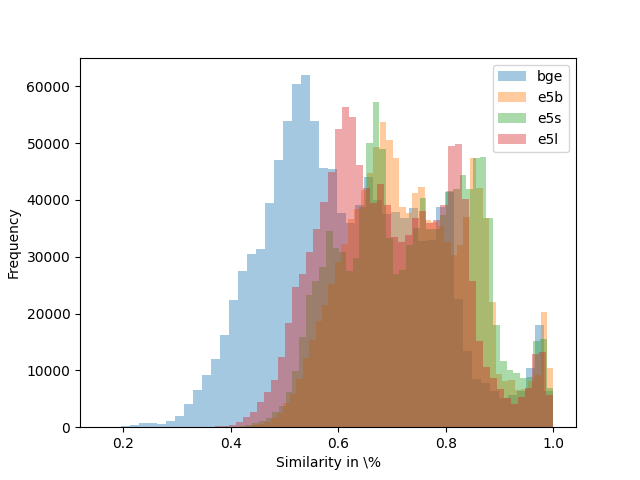
\includegraphics[width=0.45\textwidth]{figures/similarity_hist_all.png}
    \end{subfigure}
    \hfill
    \begin{subfigure}{b}
        \centering
        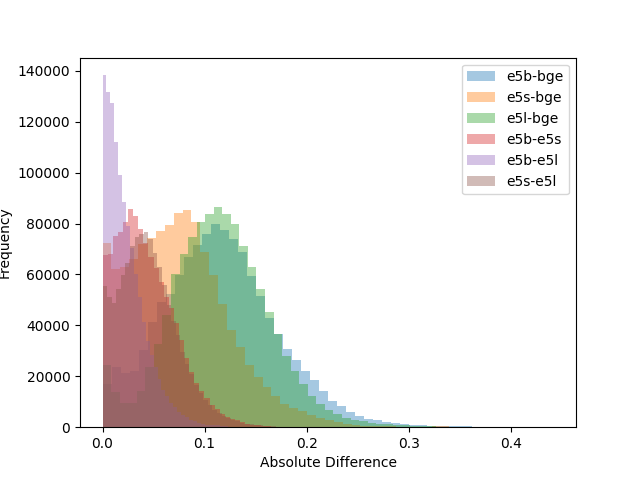
\includegraphics[width=0.45\textwidth]{figures/dissimilarity_all.png}
    \end{subfigure}
    \begin{subfigure}{b}
        \centering
        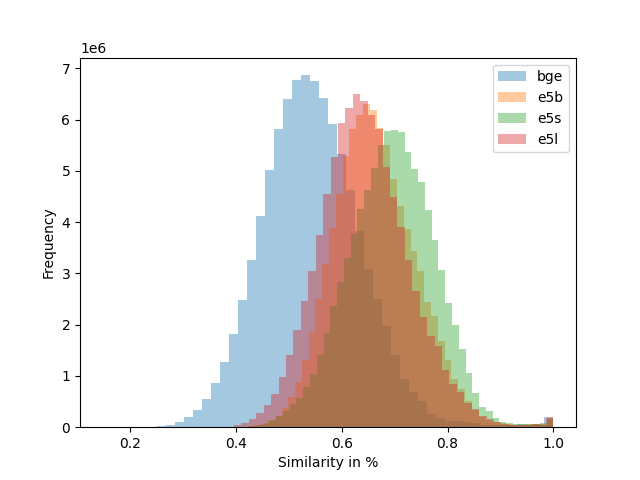
\includegraphics[width=0.45\textwidth]{figures/similarity_hist_all_pages.png}
    \end{subfigure}
    \hfill
    \begin{subfigure}{b}
        \centering
        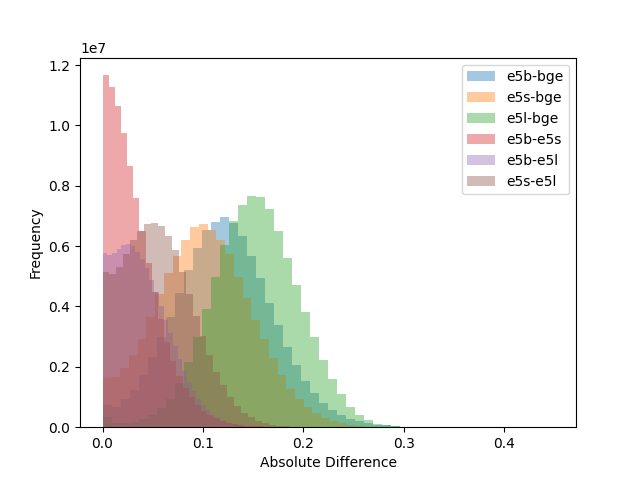
\includegraphics[width=0.45\textwidth]{figures/dissimilarity_all_pages.png}
    \end{subfigure}
\end{figure}

Based on our analysis of the different chunking strategies, we settled on computing file embeddings as the averaged embeddings of the pages within the file.
With this strategy, we recorded the total time to create the embeddings for each embedding model, along with the resulting size of the embeddings, presented in \autoref{tab:embedding_metrics}.
As expected, the quickest ingestion time was achieved with the \texttt{e5-nl-small-trm} model, while the longest times were recorded for the \texttt{bge-m3} and \texttt{e5-nl-large-trm} models.
The size of the embeddings followed the same trend.

\begin{table}[h!]
    \centering
    \begin{tabular}{l|c |c | c| c}
        model & No. Params & Dim Embedding & Time (min.s) & Size (mb) \\
        bge-m3 & & & 68.30 & 44\\
        e5-nl-small-trm & & & 9.24 & 16.7\\
        e5-nl-base-trm & & & 23.50 & 33.1 \\
        e5-nl-large-trm & & & 58.32 & 44 \\
    \end{tabular}
    \caption{Metrics for the creation of embeddings for each tested embedding model. From left to right, time required to create the embeddings for the whole dataset, size of the embeddings, and the similarity of the embeddings (mean, std) are given.}
    \label{tab:embeddings_metrics}
\end{table}


\subsubsection{Energy and Computational Cost}

\subsection{Retrieval}



\begin{table}[h!]
    \centering
    \begin{tabular}{c|c}
        retrieval time & bm25 & bge-m3  & e5-small & e5-base & e5-large\\
        \text{'road construction drawing'} & 
    \end{tabular}
    \caption{Caption}
    \label{tab:placeholder}
\end{table}

- 'road construction drawing', k=20: 39ms

pure semantic
- 'road construction drawing', k=20: 19.46s


hybrid
- 'road construction drawing', k=20: 5.98s